\PassOptionsToPackage{numbers}{natbib}
\documentclass{tufte-handout}
\usepackage{pgfplots}
\usepackage[dvipsnames]{xcolor}
\usepackage{ulem}
\usepackage{subcaption}
\usepackage{amssymb, amsmath, pgfplots, tabularx, siunitx}
\usepackage{algorithm}
\usepackage{algorithmic}
\usepackage{makecell}
\usepackage{amsfonts}
\usepackage{pgfplots}
\usepackage[dvipsnames]{xcolor}
\usepackage{amsmath, amssymb, amsthm}
\usepackage{mathtools}
\usepackage{bm}
\usepackage{thmtools}
\usepackage{enumitem}
\usepackage{graphicx}
\usepackage{caption}
\usepackage{subcaption}
\usepackage{tikz}
\usetikzlibrary{calc,arrows.meta,patterns}

\pgfplotsset{compat = newest}

\usepackage{tikz}
\usetikzlibrary{shadings}
\usetikzlibrary{calc,arrows.meta}
\usetikzlibrary{shapes.misc}
\usepackage[most]{tcolorbox}
\usepgfplotslibrary{colormaps,patchplots}

\definecolor{wp-bg}{HTML}{FDF6EF}
\definecolor{wp-text}{HTML}{2D1B0E}
\definecolor{wp-primary}{HTML}{C24A3A}
\definecolor{wp-accent}{HTML}{D4952E}
\definecolor{wp-light}{HTML}{F0DECA}
\definecolor{wp-muted}{HTML}{C4A88A}
\definecolor{wp-dark}{HTML}{1A0F07}
\definecolor{wp-code}{HTML}{FDF2E4}

\pagecolor{wp-bg}
\color{wp-text}

\hypersetup{colorlinks=true,linkcolor=wp-primary,urlcolor=wp-accent}

\declaretheorem[style=plain, name=Definition, numberwithin=section]{defn}
\declaretheorem[style=plain, name=Theorem, numberwithin=section]{thm}
\declaretheorem[style=plain, name=Lemma, numberwithin=section]{lem}
\declaretheorem[style=remark, name=Example, numberwithin=section]{exmp}
\declaretheorem[style=plain, name=Theorem, numberwithin=section]{theorem}
\declaretheorem[style=remark, name=Remark, numberwithin=section]{remark}


\tikzset{basic/.style={draw,text width=1em,text badly centered}}
\tikzset{input/.style={basic,circle}}
\tikzset{weights/.style={basic,rectangle}}
\tikzset{functions/.style={basic,circle}}

\title{Machine Learning Notes \\ Preliminary Introduction to Deep Learning}
\author{Vitor N. Cabral de Oliveira\\ \href{mailto:vnco@cin.ufpe.br}{vnco@cin.ufpe.br}}
\date{December 2024}

\begin{document}

\maketitle
\begin{abstract}
    This notebook serves as a comprehensive repository for my Machine Learning studies, with a primary focus on Deep Learning. Key topics covered include:
    \begin{itemize}
        \item Foundations of statistical learning.
        \item Artificial Neural Networks (ANNs) – Fundamentals and architectures with mathematical explanation.
    \end{itemize}
\end{abstract}

\newpage
\hypersetup{linkcolor=wp-text}
\tableofcontents
\hypersetup{linkcolor=wp-primary}
\newpage

\section{Preliminary Foundations of Statistical Learning}

Before diving into neural network architectures, it is essential to establish the fundamental concepts of statistical learning theory. This framework formalizes the problem of learning from data and provides the theoretical basis for algorithms such as the perceptron and multilayer networks.

\subsection{The Learning Problem}

In supervised learning, we are given a training set $\mathcal{D} = \{(\mathbf{x}_i, y_i)\}_{i=1}^{N}$, where each $\mathbf{x}_i \in \mathcal{X} \subseteq \mathbb{R}^d$ is an input vector (feature vector) and $y_i \in \mathcal{Y}$ is the corresponding target output. The nature of $\mathcal{Y}$ defines the task:
\begin{itemize}
    \item \textbf{Classification:} $\mathcal{Y} = \{1,\dots, K\}$ (finite set of class labels).
    \item \textbf{Regression:} $\mathcal{Y} = \mathbb{R}$ (real-valued output).
\end{itemize}

The fundamental assumption is that the training examples are drawn independently and identically distributed (i.i.d.) from an unknown joint probability distribution $P(\mathbf{x}, y)$ over $\mathcal{X} \times \mathcal{Y}$.

\subsection{Hypothesis Space and Loss Functions}

A learning algorithm selects a hypothesis $h: \mathcal{X} \to \mathcal{Y}$ from a predefined hypothesis space $\mathcal{H}$. The quality of a hypothesis is measured by a \textbf{loss function} $\ell: \mathcal{Y} \times \mathcal{Y} \to \mathbb{R}_{\ge 0}$, where $\ell(h(\mathbf{x}), y)$ quantifies the cost of predicting $h(\mathbf{x})$ when the true target is $y$. Common loss functions include:
\begin{itemize}
    \item \textbf{0–1 loss (classification):} $\ell(h(\mathbf{x}), y) = \mathbf{1}_{h(\mathbf{x}) \neq y}$.
    \item \textbf{Squared loss (regression):} $\ell(h(\mathbf{x}), y) = (y - h(\mathbf{x}))^2$.
    \item \textbf{Cross-entropy loss (classification with probabilities):} $\ell(\hat{\mathbf{p}}, y) = -\sum_{k=1}^K \mathbf{1}_{y=k} \log \hat{p}_k$.
\end{itemize}

The ultimate goal is to minimize the \textbf{expected risk} (also called true risk or generalization error):
\begin{equation}
    R(h) = \mathbb{E}_{(\mathbf{x}, y) \sim P} \left[ \ell(h(\mathbf{x}), y) \right].
\end{equation}
Since $P$ is unknown, we cannot directly compute $R(h)$. Instead, we minimize the \textbf{empirical risk} over the training set:
\begin{equation}
    \widehat{R}_{\mathcal{D}}(h) = \frac{1}{N} \sum_{i=1}^{N} \ell(h(\mathbf{x}_i), y_i).
\end{equation}

\subsection{Empirical Risk Minimization (ERM)}

The principle of empirical risk minimization (ERM) \cite{Vapnik1998} selects the hypothesis that minimizes the empirical risk:
\begin{equation}
    h_{\text{ERM}} = \arg\min_{h \in \mathcal{H}} \widehat{R}_{\mathcal{D}}(h).
\end{equation}
For finite $\mathcal{H}$, uniform convergence bounds (e.g., Hoeffding's inequality together with union bound) guarantee that with high probability, $R(h_{\text{ERM}})$ is close to the minimal possible risk $\min_{h \in \mathcal{H}} R(h)$, provided the sample size $N$ is sufficiently large relative to the complexity of $\mathcal{H}$. This interplay between approximation error (bias) and estimation error (variance) is captured by the \textbf{bias–variance decomposition} (for squared loss):
\begin{equation}
    \mathbb{E}_{\mathcal{D}} \left[ R(h_{\mathcal{D}}) \right] = \underbrace{R(h^*)}_{\text{irreducible error}} + \underbrace{\left( \mathbb{E}_{\mathcal{D}}[h_{\mathcal{D}}] - h^* \right)^2}_{\text{bias}^2} + \underbrace{\mathbb{V}_{\mathcal{D}}[h_{\mathcal{D}}]}_{\text{variance}}.
\end{equation}
where $h^*$ is the Bayes-optimal hypothesis. Larger hypothesis spaces reduce bias but increase variance, leading to the classic \textbf{bias–variance tradeoff}.

\subsection{Stochastic Gradient Descent as an Optimization Method}

Most modern machine learning models, including neural networks, are trained by minimizing the empirical risk using gradient-based optimization. Because the empirical risk is an average over $N$ terms,
\[
\widehat{R}_{\mathcal{D}}(\mathbf{w}) = \frac{1}{N} \sum_{i=1}^N \ell_i(\mathbf{w}),
\]
the full gradient $\nabla \widehat{R}_{\mathcal{D}}(\mathbf{w})$ requires a pass through the entire dataset, which is computationally expensive for large $N$. The stochastic gradient descent (SGD) algorithm replaces the true gradient by an unbiased estimate computed from a mini‑batch of examples:
\[
\mathbf{w}_{t+1} = \mathbf{w}_t - \eta_t \cdot \frac{1}{|\mathcal{B}|} \sum_{i \in \mathcal{B}} \nabla \ell_i(\mathbf{w}_t),
\]
where $\mathcal{B} \subset \{1,\dots,N\}$ is a random mini‑batch. This stochastic approximation introduces noise but enables efficient optimisation, especially for large‑scale problems.

With these foundations in place, we now turn to the earliest and simplest learnable model: the perceptron.



%%%%%%%%%%%%%%%%%%%%%%%%%%%%%%%%%%%%%%%%%%%%%%%%%%%%

\section{Probability Spaces and Axioms}

Probability theory begins with a mathematical model for random experiments. The fundamental structure is the \textbf{probability space}.

\begin{defn}[Probability Space]
    A probability space is a triple $(\Omega, \mathcal{F}, P)$ where:
    \begin{enumerate}[label=(\roman*)]
        \item $\Omega$ is a nonempty set, called the \textbf{sample space}. Its elements $\omega \in \Omega$ are elementary outcomes.
        \item $\mathcal{F}$ is a $\sigma$-\textbf{algebra} (or $\sigma$-field) of subsets of $\Omega$: a collection of subsets containing $\Omega$, closed under complement and countable union. The elements $A \in \mathcal{F}$ are called \textbf{events}.
        \item $P: \mathcal{F} \to [0,1]$ is a \textbf{probability measure} satisfying the Kolmogorov axioms:
            \begin{enumerate}
                \item $P(A) \ge 0$ for all $A \in \mathcal{F}$.
                \item $P(\Omega) = 1$.
                \item If $A_1, A_2, \dots$ are pairwise disjoint ($A_i \cap A_j = \varnothing$ for $i \ne j$), then
                \[
                P\!\left(\bigcup_{i=1}^{\infty} A_i\right) = \sum_{i=1}^{\infty} P(A_i) \quad \text{($\sigma$-additivity)}.
                \]
                \end{enumerate}
            \end{enumerate}
\end{defn}

\begin{marginfigure}
\centering
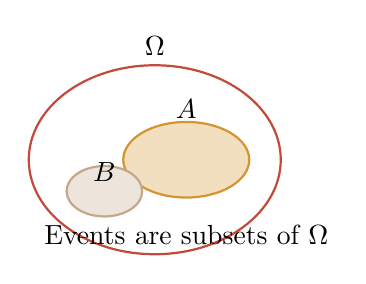
\begin{tikzpicture}[scale=0.8]
    \draw[thick, wp-primary] (0,0) ellipse (2 and 1.5);
    \node at (0,1.8) {$\Omega$};
    \fill[wp-accent!30, draw=wp-accent, thick] (0.5,0) ellipse (1 and 0.6);
    \node at (0.5,0.8) {$A$};
    \fill[wp-muted!30, draw=wp-muted, thick] (-0.8,-0.5) ellipse (0.6 and 0.4);
    \node at (-0.8,-0.2) {$B$};
    \node at (0.5,-1.2) {Events are subsets of $\Omega$};
\end{tikzpicture}
\caption{A sample space $\Omega$ with two events $A$ and $B$.}
\end{marginfigure}

The $\sigma$-algebra $\mathcal{F}$ formalizes which subsets of $\Omega$ are considered measurable (i.e., we can assign a probability). In discrete settings we often take $\mathcal{F} = 2^{\Omega}$ (all subsets). For continuous spaces like $\mathbb{R}$, we use the Borel $\sigma$-algebra generated by open intervals.

\subsection{Properties of Probability Measures}

From the axioms we derive several useful properties:
\begin{itemize}
    \item $P(\varnothing) = 0$.
    \item Finite additivity: for disjoint $A_1,\dots,A_n$, $P(\bigcup_{i=1}^n A_i) = \sum_{i=1}^n P(A_i)$.
    \item Monotonicity: If $A \subseteq B$, then $P(A) \le P(B)$.
    \item Complement: $P(A^c) = 1 - P(A)$.
    \item Union bound (Boole's inequality): $P(\bigcup_i A_i) \le \sum_i P(A_i)$.
    \item Inclusion–exclusion: $P(A \cup B) = P(A) + P(B) - P(A \cap B)$.
\end{itemize}

\subsection{Conditional Probability and Independence}

Conditional probability quantifies how the probability of an event changes given that another event has occurred.

\begin{defn}[Conditional Probability]
    For events $A$ and $B$ with $P(B) > 0$, the conditional probability of $A$ given $B$ is
    \[
    P(A \mid B) = \frac{P(A \cap B)}{P(B)}.
    \]
\end{defn}

\begin{defn}[Independence]
    Two events $A$ and $B$ are \textbf{independent} if $P(A \cap B) = P(A)P(B)$. Equivalently, $P(A \mid B) = P(A)$ when $P(B)>0$. A collection $\{A_i\}$ is mutually independent if for every finite subset $I$,
    \[
    P\!\left(\bigcap_{i \in I} A_i\right) = \prod_{i \in I} P(A_i).
    \]
\end{defn}

\paragraph{Bayes' Theorem}
A fundamental result that reverses conditioning:
\[
P(A \mid B) = \frac{P(B \mid A) P(A)}{P(B)}, \qquad \text{where } P(B) = \sum_i P(B \mid A_i)P(A_i)
\]
for a partition $\{A_i\}$ of $\Omega$. Bayes' theorem is the cornerstone of Bayesian inference and permeates modern machine learning (e.g., naive Bayes classifiers, Bayesian neural networks).

\begin{marginfigure}
\centering
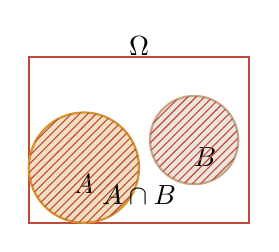
\begin{tikzpicture}[scale=0.7]
    \draw[thick, wp-primary] (0,0) rectangle (4,3);
    \node at (2,3.2) {$\Omega$};
    \fill[wp-accent!30, draw=wp-accent, thick] (1,1) circle (1);
    \node at (1,0.7) {$A$};
    \fill[wp-muted!30, draw=wp-muted, thick] (3,1.5) circle (0.8);
    \node at (3.2,1.2) {$B$};
    \fill[pattern=north east lines, pattern color=wp-primary] (1,1) circle (1) (3,1.5) circle (0.8);
    \node at (2,0.5) {$A \cap B$};
\end{tikzpicture}
\caption{Bayes' theorem relates $P(A|B)$ to $P(B|A)$ via the prior $P(A)$ and evidence $P(B)$.}
\end{marginfigure}

\section{Random Variables}

Often we are not directly interested in elementary outcomes but in numerical quantities derived from them.

\begin{defn}[Random Variable]
    A \textbf{random variable} $X$ on a probability space $(\Omega,\mathcal{F},P)$ is a function $X: \Omega \to \mathbb{R}$ such that for every Borel set $B \subseteq \mathbb{R}$, the preimage $X^{-1}(B) = \{\omega: X(\omega) \in B\}$ belongs to $\mathcal{F}$ (i.e., $X$ is \textit{measurable}). This condition ensures that probabilities of events involving $X$ are well-defined.
\end{defn}

\subsection{Discrete and Continuous Random Variables}

\begin{itemize}
    \item \textbf{Discrete} $X$ takes values in a countable set $\mathcal{X} \subseteq \mathbb{R}$. It is described by its \textbf{probability mass function (PMF)} $p_X(x) = P(X = x)$.
    \item \textbf{Continuous} $X$ has a \textbf{probability density function (PDF)} $f_X(x)$ such that for any interval $[a,b]$,
    \[
    P(a \le X \le b) = \int_a^b f_X(x)\,dx.
    \]
    The PDF satisfies $f_X(x) \ge 0$ and $\int_{-\infty}^{\infty} f_X(x)\,dx = 1$.
\end{itemize}

The \textbf{cumulative distribution function (CDF)} $F_X(x) = P(X \le x)$ is defined for any random variable and is non‑decreasing, right‑continuous, with $\lim_{x\to-\infty}F_X(x)=0$, $\lim_{x\to\infty}F_X(x)=1$.

\begin{marginfigure}
\centering
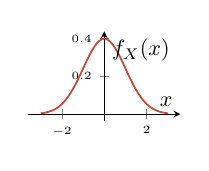
\begin{tikzpicture}[scale=0.8]
    \begin{axis}[width=4cm, height=3cm, xlabel=$x$, ylabel=$f_X(x)$, domain=-3:3, samples=100, axis lines=middle, enlargelimits, ticklabel style={font=\tiny}]
        \addplot[wp-primary, thick] {exp(-x^2/2)/sqrt(2*pi)};
    \end{axis}
\end{tikzpicture}
\caption{PDF of the standard normal distribution.}
\end{marginfigure}

\section{Expectation and Moments}

The expectation (mean) is the weighted average of a random variable.

\begin{defn}[Expectation]
    For a discrete random variable $X$ with PMF $p_X$, $\mathbb{E}[X] = \sum_{x} x\, p_X(x)$ (provided the sum converges absolutely). For continuous $X$ with PDF $f_X$, $\mathbb{E}[X] = \int_{-\infty}^{\infty} x\, f_X(x)\,dx$.
\end{defn}

\paragraph{Properties of Expectation}
\begin{itemize}
    \item Linearity: $\mathbb{E}[aX + bY] = a\mathbb{E}[X] + b\mathbb{E}[Y]$ for constants $a,b$.
    \item If $X \ge 0$ almost surely, then $\mathbb{E}[X] \ge 0$.
    \item Law of the unconscious statistician: $\mathbb{E}[g(X)] = \sum_x g(x)p_X(x)$ (discrete) or $\int g(x)f_X(x)\,dx$ (continuous).
\end{itemize}

\subsection{Variance and Covariance}

\begin{defn}[Variance]
    The variance of $X$ measures its spread around the mean:
    \[
    \operatorname{Var}(X) = \mathbb{E}\bigl[(X - \mathbb{E}[X])^2\bigr] = \mathbb{E}[X^2] - (\mathbb{E}[X])^2.
    \]
    The standard deviation is $\sigma_X = \sqrt{\operatorname{Var}(X)}$.
\end{defn}

\begin{defn}[Covariance and Correlation]
    For two random variables $X,Y$,
    \[
    \operatorname{Cov}(X,Y) = \mathbb{E}\bigl[(X - \mathbb{E}[X])(Y - \mathbb{E}[Y])\bigr] = \mathbb{E}[XY] - \mathbb{E}[X]\mathbb{E}[Y].
    \]
    The correlation coefficient is $\rho(X,Y) = \frac{\operatorname{Cov}(X,Y)}{\sigma_X \sigma_Y}$, satisfying $-1 \le \rho \le 1$.
\end{defn}

If $X$ and $Y$ are independent, then $\operatorname{Cov}(X,Y)=0$ (the converse is not true in general).

\section{Important Distributions for Machine Learning}

Several probability distributions appear repeatedly in machine learning.

\subsection{Bernoulli and Binomial}
\begin{itemize}
    \item \textbf{Bernoulli}$(\theta)$: $X \in \{0,1\}$, $P(X=1)=\theta$, $P(X=0)=1-\theta$. $\mathbb{E}[X]=\theta$, $\operatorname{Var}(X)=\theta(1-\theta)$. Used for binary classification.
    \item \textbf{Binomial}$(n,\theta)$: $X = \sum_{i=1}^n Y_i$ with $Y_i$ i.i.d. Bernoulli$(\theta)$. PMF: $P(X=k) = \binom{n}{k}\theta^k(1-\theta)^{n-k}$, $\mathbb{E}[X]=n\theta$, $\operatorname{Var}(X)=n\theta(1-\theta)$.
\end{itemize}

\subsection{Gaussian (Normal) Distribution}
The most ubiquitous continuous distribution.
\[
\mathcal{N}(\mu, \sigma^2):\quad f(x) = \frac{1}{\sqrt{2\pi\sigma^2}} \exp\!\left(-\frac{(x-\mu)^2}{2\sigma^2}\right),\quad \mathbb{E}[X]=\mu,\ \operatorname{Var}(X)=\sigma^2.
\]
The standard normal $\mathcal{N}(0,1)$ has mean $0$ and variance $1$. By the Central Limit Theorem, sums of many independent random variables tend to a Gaussian.

\subsection{Exponential and Laplace}
\begin{itemize}
    \item \textbf{Exponential}$(\lambda)$: $f(x) = \lambda e^{-\lambda x}$, $x \ge 0$, $\mathbb{E}[X]=1/\lambda$. Used for waiting times.
    \item \textbf{Laplace}$(\mu,b)$: $f(x) = \frac{1}{2b}\exp\!\left(-\frac{|x-\mu|}{b}\right)$. Heavier tails than Gaussian; used in robust regression.
\end{itemize}

\subsection{Multivariate Gaussian}
For a random vector $\mathbf{X} = (X_1,\dots,X_d)^{\mathsf{T}}$,
\[
\mathcal{N}(\boldsymbol{\mu}, \boldsymbol{\Sigma}):\quad f(\mathbf{x}) = \frac{1}{(2\pi)^{d/2}|\boldsymbol{\Sigma}|^{1/2}} \exp\!\left(-\frac{1}{2}(\mathbf{x}-\boldsymbol{\mu})^{\mathsf{T}}\boldsymbol{\Sigma}^{-1}(\mathbf{x}-\boldsymbol{\mu})\right),
\]
with mean vector $\boldsymbol{\mu} \in \mathbb{R}^d$ and positive‑definite covariance matrix $\boldsymbol{\Sigma}$. This is the foundation of many latent variable models and deep generative models (e.g., variational autoencoders).

\section{Limit Theorems}

These theorems justify why averaging works and why the Gaussian distribution appears so often.

\begin{thm}[Law of Large Numbers (LLN)]
    Let $X_1, X_2, \dots$ be i.i.d. with $\mathbb{E}[X_i] = \mu$. Then the sample average $\overline{X}_n = \frac{1}{n}\sum_{i=1}^n X_i$ converges to $\mu$ in probability:
    \[
    \forall \varepsilon >0,\quad \lim_{n\to\infty} P(|\overline{X}_n - \mu| > \varepsilon) = 0.
    \]
\end{thm}

\begin{thm}[Central Limit Theorem (CLT)]
    Under the same i.i.d. assumption with finite variance $\sigma^2$, the scaled sample average converges in distribution to a standard normal:
    \[
    \sqrt{n}\,\frac{\overline{X}_n - \mu}{\sigma} \xrightarrow{d} \mathcal{N}(0,1).
    \]
    Equivalently, $\overline{X}_n \approx \mathcal{N}(\mu, \sigma^2/n)$ for large $n$.
\end{thm}

\begin{marginfigure}
\centering
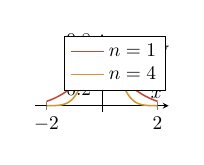
\begin{tikzpicture}[scale=0.7]
    \begin{axis}[width=4cm, height=3cm, xlabel=$\overline{x}$, ylabel=density, domain=-2:2, samples=100, axis lines=middle, enlargelimits]
        \addplot[wp-primary, thick] {exp(-x^2/2)/sqrt(2*pi)};
        \addplot[wp-accent, thick, domain=-2:2] {exp(-x^2/(2*0.25))/sqrt(2*pi*0.25)};
        \legend{$n=1$, $n=4$};
    \end{axis}
\end{tikzpicture}
\caption{The CLT: as $n$ increases, the distribution of $\overline{X}_n$ becomes narrower and more Gaussian.}
\end{marginfigure}

The CLT explains why the Gaussian prior is a common choice and why many estimators are asymptotically normal.

\section{Multivariate Random Vectors and Joint Distributions}

When dealing with multiple random variables simultaneously, we use the joint distribution.

\begin{defn}[Joint PDF/PMF]
    For a random vector $(X_1,\dots,X_d)$:
    \begin{itemize}
        \item Discrete: joint PMF $p(x_1,\dots,x_d) = P(X_1=x_1,\dots,X_d=x_d)$.
        \item Continuous: joint PDF $f(x_1,\dots,x_d)$ satisfying $P(\mathbf{X} \in A) = \int_A f(\mathbf{x})\,d\mathbf{x}$.
    \end{itemize}
\end{defn}

\subsection{Marginal and Conditional Distributions}
\begin{itemize}
    \item \textbf{Marginal} PMF/PDF: e.g., $p_{X_1}(x_1) = \sum_{x_2,\dots,x_d} p(x_1,\dots,x_d)$ (discrete) or $f_{X_1}(x_1) = \int \cdots \int f(x_1,\dots,x_d)\,dx_2\cdots dx_d$ (continuous).
    \item \textbf{Conditional} distribution of $X$ given $Y=y$: $f_{X|Y}(x|y) = \frac{f_{X,Y}(x,y)}{f_Y(y)}$ (for continuous) and similarly for PMF.
\end{itemize}

\subsection{Independence of Random Variables}
Random variables $X_1,\dots,X_d$ are independent iff their joint distribution factorizes:
\[
f(x_1,\dots,x_d) = \prod_{i=1}^d f_{X_i}(x_i) \quad (\text{or PMF analog}).
\]
Independence simplifies many computations and is a common modeling assumption (e.g., naive Bayes).

\subsection{Law of Total Expectation and Variance}
For two random variables $X,Y$,
\[
\mathbb{E}[X] = \mathbb{E}\bigl[\mathbb{E}[X \mid Y]\bigr],\qquad
\operatorname{Var}(X) = \mathbb{E}\bigl[\operatorname{Var}(X \mid Y)\bigr] + \operatorname{Var}\bigl(\mathbb{E}[X \mid Y]\bigr).
\]
These identities are crucial in deriving algorithms like expectation–maximization and in analyzing stochastic gradient descent.

\section{Information Theory for Machine Learning}

Information theory provides tools to quantify uncertainty and information content, which are essential for understanding entropy, cross‑entropy loss, and Kullback–Leibler divergence.

\begin{defn}[Entropy]
    For a discrete random variable $X$ with PMF $p$, the \textbf{Shannon entropy} is
    \[
    H(X) = -\sum_{x} p(x) \log p(x),
    \]
    measured in bits if the logarithm is base 2, or nats if natural log. Entropy measures the average uncertainty about $X$.
\end{defn}

\begin{defn}[Kullback–Leibler Divergence]
    For two probability distributions $p$ and $q$ over the same alphabet,
    \[
    D_{\text{KL}}(p \parallel q) = \sum_x p(x) \log\frac{p(x)}{q(x)}
    \]
    (with $0\log0=0$). $D_{\text{KL}}$ is non‑negative and zero iff $p=q$. It is asymmetric and measures how much information is lost when $q$ approximates $p$.
\end{defn}

The cross‑entropy between $p$ and $q$ is $H(p,q) = H(p) + D_{\text{KL}}(p\parallel q) = -\sum_x p(x)\log q(x)$. Minimizing cross‑entropy is equivalent to minimizing KL divergence when $p$ is fixed (the true distribution) – this is exactly what many classification neural networks do (categorical cross‑entropy loss).

\begin{marginfigure}
\centering
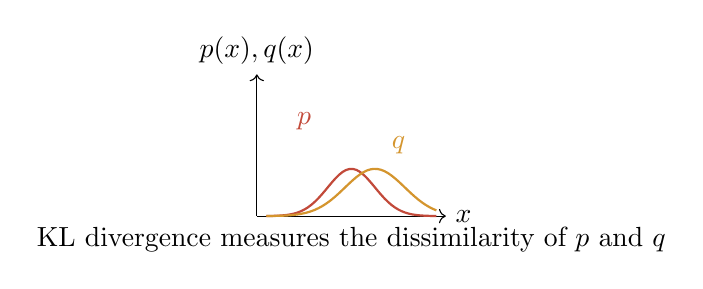
\begin{tikzpicture}[scale=0.6]
    \draw[->] (0,0) -- (4,0) node[right] {$x$};
    \draw[->] (0,0) -- (0,3) node[above] {$p(x), q(x)$};
    \draw[wp-primary, thick, domain=0.2:3.8, samples=50] plot (\x, {exp(-(\x-2)^2/0.5)});
    \draw[wp-accent, thick, domain=0.2:3.8, samples=50] plot (\x, {exp(-(\x-2.5)^2/0.8)});
    \node[wp-primary] at (1,2) {$p$};
    \node[wp-accent] at (3,1.5) {$q$};
    \node at (2,-0.5) {KL divergence measures the dissimilarity of $p$ and $q$};
\end{tikzpicture}
\caption{KL divergence $D_{\text{KL}}(p\parallel q)$ is zero when the distributions coincide.}
\end{marginfigure}

%%%%%%%%%%%%%%%%%%%%%%%%%%%%%%%%%%%%%%%%%%%%%%%%%%%%

\section{Introduction to Artificial Neural Networks}

\subsection{Perceptron}

Nearly every modern artificial neural network, from simple classifiers to sprawling deep learning architectures, traces its origins to a simple computational unit called the \textbf{perceptron} \sidenote[1]{While most neural networks rely on perceptron-like units, alternative paradigms exist, such as Hebbian learning (inspired by synaptic plasticity) and the recently revived Kolmogorov–Arnold Network (KAN), which bypasses traditional neuron structures entirely.}.

Developed by Frank Rosenblatt in 1947, inspired by the work of McCulloch and Pitts in 1943. The perceptron, sometimes called the \textit{sigmoid neuron}, it's traced back from the mathematical interpretation of the biological neurons' way of functioning.

At its core, the perceptron is a binary decision-maker. It takes a set of real-valued inputs, weighs their importance, and makes a crisp, threshold-based choice.

\paragraph{Mathematical Definition}

Given inputs $x_1, x_2, \dots, x_n \in \mathbb{R}$, the perceptron's output is defined by:
\begin{enumerate}
    \item \textbf{Weighted sum (affine transformation):}
    \begin{equation}
        z = w_0 + \sum_{i=1}^{n} w_i x_i,
    \end{equation}
    where $w_i \in \mathbb{R}$ are the \textit{weights} and $w_0$ is the \textit{bias term}.
    \item \textbf{Thresholding (activation):}
    \begin{equation}\label{eq:perceptron}
        o(\mathbf{x}) = \phi(z) = 
        \begin{cases}
            1, & \text{if } z > 0,\\
            0, & \text{otherwise}.
        \end{cases}
    \end{equation}
\end{enumerate}
By introducing a dummy input $x_0 = 1$, we can absorb the bias into the weight vector: let $\mathbf{w} = (w_0, w_1, \dots, w_n)^{\mathsf{T}} \in \mathbb{R}^{n+1}$ and $\mathbf{x} = (1, x_1, \dots, x_n)^{\mathsf{T}}$. Then $z = \mathbf{w} \cdot \mathbf{x}$ and the output is $o(\mathbf{x}) = \mathbf{1}_{\mathbf{w} \cdot \mathbf{x} > 0}$.

\paragraph{Geometric Interpretation}

The decision boundary is the hyperplane $\{\mathbf{x} \in \mathbb{R}^{n+1} : \mathbf{w} \cdot \mathbf{x} = 0\}$ that separates the input space into two half‑spaces. For $n = 2$, this reduces to a line:
\[
w_0 + w_1 x_1 + w_2 x_2 = 0,
\]
with slope determined by $-w_1/w_2$ and intercept by $-w_0/w_2$. The weight vector $\mathbf{w}$ is orthogonal to this decision boundary and points towards the region where $\mathbf{w} \cdot \mathbf{x} > 0$.

\begin{marginfigure}
\centering
    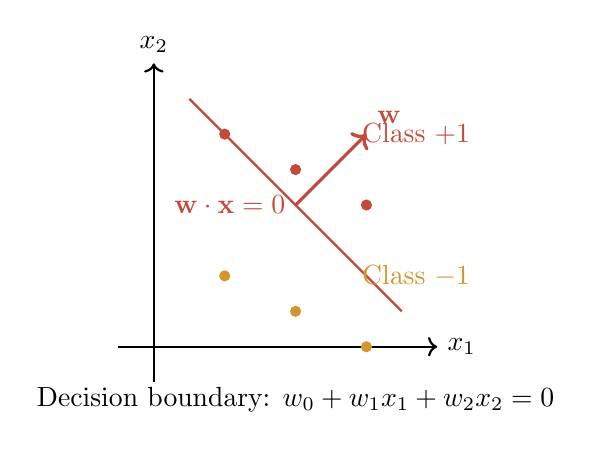
\begin{tikzpicture}[scale=0.9]

    % Axes
    \draw[->, thick] (-0.5,0) -- (4,0) node[right]{$x_1$};
    \draw[->, thick] (0,-0.5) -- (0,4) node[above]{$x_2$};

    % Decision boundary (w0 + w1x1 + w2x2 = 0)
    \draw[wp-primary, thick] (0.5,3.5) -- (3.5,0.5) node[midway, left]{$\mathbf{w}\cdot\mathbf{x}=0$};

    % Weight vector (normal to boundary)
    \draw[->, wp-primary, very thick] (2,2) -- (3,3) node[above right]{$\mathbf{w}$};
    \filldraw[wp-primary] (1,3) circle (2pt);
    \filldraw[wp-primary] (2,2.5) circle (2pt);
    \filldraw[wp-primary] (3,2) circle (2pt);
    \filldraw[wp-accent] (1,1) circle (2pt);
    \filldraw[wp-accent] (2,0.5) circle (2pt);
    \filldraw[wp-accent] (3,0) circle (2pt);
    \node[wp-primary] at (3.7,3) {Class $+1$};
    \node[wp-accent] at (3.7,1) {Class $-1$};

    \node at (2,-0.75) {Decision boundary: $w_0 + w_1x_1 + w_2x_2 = 0$};

\end{tikzpicture}
\end{marginfigure}

The perceptron can only represent \textit{linearly separable} functions. The classic XOR problem (Figure~\ref{fig:xor_combined}) is not linearly separable, which motivated the development of multilayer architectures.

\begin{figure}[h]
    \centering
    \begin{subfigure}{0.45\textwidth}
        \centering
        \begin{tabular}{c|c|c}
            $x_1$ & $x_2$ & $x_1 \oplus x_2$ \\
            \hline
            0 & 0 & 0 \\
            1 & 0 & 1 \\
            0 & 1 & 1 \\
            1 & 1 & 0 \\
        \end{tabular}
        \caption{XOR truth table}
        \label{tab:xor}
    \end{subfigure}
    \begin{subfigure}{0.45\textwidth}
        \centering
        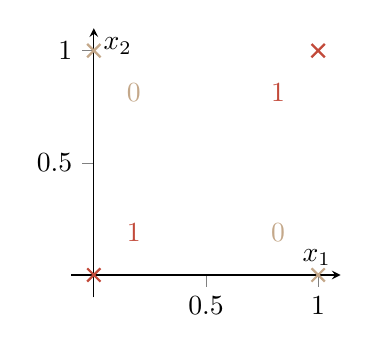
\begin{tikzpicture}
            \tikzstyle{point}=[thick,draw=wp-text,cross out,inner sep=0pt,minimum width=4pt,minimum height=4pt]
            \begin{axis}[
                legend pos=south west,
                axis x line=middle,
                axis y line=middle,
                grid=none,
                width=5cm,
                height=5cm,
                grid style={dashed, wp-muted!30},
                xmin=0, xmax=1, ymin=0, ymax=1,
                xlabel=$x_1$,
                ylabel=$x_2$,
                tick align=outside,
                enlargelimits=true]
              \node[point,label={[label distance=0.3cm,text=wp-muted]135:$0$},wp-muted] at (axis cs:1,0) {};
              \node[point,label={[label distance=0.3cm,text=wp-muted]-45:$0$},wp-muted] at (axis cs:0,1) {};
              \node[point,label={[label distance=0.3cm,text=wp-primary]45:$1$},wp-primary] at (axis cs:0,0) {};
              \node[point,label={[label distance=0.3cm,text=wp-primary]-135:$1$},wp-primary] at (axis cs:1,1) {};
            \end{axis}
        \end{tikzpicture}
        \caption{XOR as a non‑linear classification problem}
        \label{fig:xor_plot}
    \end{subfigure}
    \caption{XOR operation: no single straight line can separate the two classes.}
    \label{fig:xor_combined}
\end{figure}

\subsection{Gradient Descent and Stochastic Gradient Descent}

\paragraph{Perceptron Training Rule}

Given a training set $\{(\mathbf{x}_d, t_d)\}_{d=1}^N$, the perceptron learning rule updates weights whenever a misclassification occurs:
\[
w_i \leftarrow w_i + \Delta w_i,\qquad \Delta w_i = \eta\, (t_d - o_d)\, x_{i,d},
\]
where $\eta > 0$ is the learning rate, $t_d$ is the target (0 or 1), $o_d$ the perceptron's output, and $x_{i,d}$ the $i$-th component of $\mathbf{x}_d$. This rule converges if the data are linearly separable; otherwise it may oscillate.

\paragraph{Delta Rule and Linear Units}

For non‑separable problems, we consider a linear unit without threshold: $o(\mathbf{x}) = \mathbf{w} \cdot \mathbf{x}$. Define the sum of squared errors over the training set:
\[
E(\mathbf{w}) = \frac{1}{2} \sum_{d=1}^{N} (t_d - o_d)^2.
\]
The gradient of $E$ with respect to $\mathbf{w}$ is
\[
\nabla_{\mathbf{w}} E(\mathbf{w}) = \sum_{d=1}^{N} (o_d - t_d)\,\mathbf{x}_d.
\]
Thus the gradient descent update is
\[
\mathbf{w} \leftarrow \mathbf{w} - \eta \nabla_{\mathbf{w}} E(\mathbf{w})
\quad\Longrightarrow\quad
\Delta w_i = \eta \sum_{d=1}^{N} (t_d - o_d)\, x_{i,d}.
\]

\paragraph{Stochastic Gradient Descent (SGD)}

For large $N$, computing the full gradient is expensive. SGD approximates it using a single random example (or a mini‑batch):
\[
\mathbf{w} \leftarrow \mathbf{w} - \eta\, (o_d - t_d)\,\mathbf{x}_d,\qquad d \sim \text{Uniform}\{1,\dots,N\}.
\]
The noisy updates allow the algorithm to escape shallow local minima and are the basis for training deep networks.

\subsection{Multilayer Perceptron and Backpropagation}

A multilayer perceptron (MLP) consists of an input layer, one or more hidden layers, and an output layer. Each neuron uses a differentiable nonlinear activation function $f(\cdot)$ (e.g., logistic sigmoid $\sigma(z) = 1/(1+e^{-z})$, hyperbolic tangent $\tanh(z)$, or ReLU $\max(0,z)$). The universal approximation theorem (Section~\ref{sec:UAT}) guarantees that MLPs with at least one hidden layer can approximate any continuous function on a compact set to arbitrary accuracy, provided enough hidden units.

\paragraph{Backpropagation Algorithm}

Let the network have $L$ layers, with weights $w_{ij}^{(\ell)}$ connecting unit $i$ in layer $\ell-1$ to unit $j$ in layer $\ell$. For an input $\mathbf{x}$, forward propagation computes:
\[
a_j^{(\ell)} = \sum_i w_{ij}^{(\ell)} o_i^{(\ell-1)},\qquad o_j^{(\ell)} = f(a_j^{(\ell)}),
\]
where $o_i^{(0)} = x_i$. The output layer produces $\hat{y}_k = o_k^{(L)}$. The loss for a single example with target $\mathbf{t}$ is, e.g., half the squared error:
\[
E = \frac{1}{2} \sum_{k \in \text{outputs}} (t_k - \hat{y}_k)^2.
\]

Backpropagation computes the gradient $\partial E / \partial w_{ij}^{(\ell)}$ via the chain rule. Define the error signal for output units:
\[
\delta_k^{(L)} = \frac{\partial E}{\partial a_k^{(L)}} = (t_k - \hat{y}_k) \, f'(a_k^{(L)}).
\]
For a hidden layer $\ell$, the error is back‑propagated:
\[
\delta_j^{(\ell)} = f'(a_j^{(\ell)}) \sum_{k} w_{jk}^{(\ell+1)} \delta_k^{(\ell+1)}.
\]
The gradient is then
\[
\frac{\partial E}{\partial w_{ij}^{(\ell)}} = \delta_j^{(\ell)} \, o_i^{(\ell-1)}.
\]
Finally, weights are updated using SGD:
\[
w_{ij}^{(\ell)} \leftarrow w_{ij}^{(\ell)} - \eta \, \delta_j^{(\ell)} o_i^{(\ell-1)}.
\]

\begin{algorithm}[h]
    \caption{Backpropagation (online version)}
    \begin{algorithmic}[1]
        \STATE Initialize all weights $w_{ij}^{(\ell)}$ randomly.
        \FOR{each training example $(\mathbf{x}, \mathbf{t})$}
            \STATE \textbf{Forward pass:} compute all $a_j^{(\ell)}$ and $o_j^{(\ell)}$.
            \STATE \textbf{Output errors:} $\delta_k^{(L)} = (t_k - o_k^{(L)}) f'(a_k^{(L)})$.
            \FOR{$\ell = L-1$ down to $1$}
                \STATE $\delta_j^{(\ell)} = f'(a_j^{(\ell)}) \sum_k w_{jk}^{(\ell+1)} \delta_k^{(\ell+1)}$.
            \ENDFOR
            \FOR{each weight $w_{ij}^{(\ell)}$}
                \STATE $w_{ij}^{(\ell)} \leftarrow w_{ij}^{(\ell)} + \eta \, \delta_j^{(\ell)} o_i^{(\ell-1)}$.
            \ENDFOR
        \ENDFOR
    \end{algorithmic}
\end{algorithm}

\subsection{Universal Approximation Theorem}
\label{sec:UAT}

One of the most important theoretical results for neural networks is the universal approximation theorem, originally proved by Cybenko (1989) for sigmoidal activation functions. The theorem states:

\begin{theorem}[Cybenko, 1989]
    Let $f: \mathbb{R}^n \to \mathbb{R}$ be any continuous function on the $n$-dimensional hypercube $[0,1]^n$. Then for any $\varepsilon > 0$, there exists a single‑hidden‑layer feedforward network with sigmoidal activation functions and a finite number of hidden units such that the network output $\hat{f}(\mathbf{x})$ satisfies
    \[
    \sup_{\mathbf{x} \in [0,1]^n} \bigl| \hat{f}(\mathbf{x}) - f(\mathbf{x}) \bigr| < \varepsilon.
    \]
\end{theorem}

The theorem implies that even a shallow network (one hidden layer) is \textit{dense} in the space of continuous functions when the number of hidden units is allowed to grow. However, it does not guarantee that such a network can be learned efficiently (the number of units may be astronomically large). Modern deep learning uses \textit{depth} to represent complex functions more compactly.

Figure~\ref{fig:UAT} illustrates the idea: a piecewise linear approximation of $\sin(x)$ improves as the number of linear regions (analogous to hidden units) increases.

\begin{figure}[h]
\centering
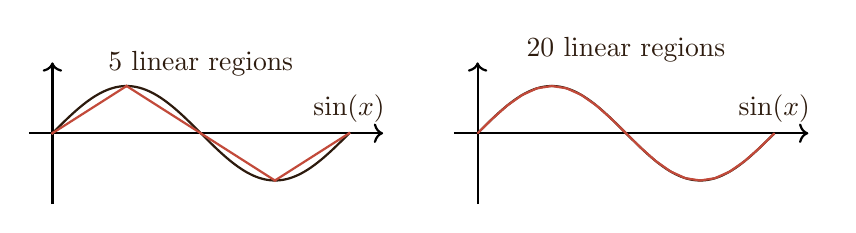
\begin{tikzpicture}[scale=.6, thick]

    % First plot: 5 linear regions
    \begin{scope}[shift={(0, 0)}]
        \draw[->] (-0.5, 0) -- (7, 0) node[right] {};
        \draw[->] (0, -1.5) -- (0, 1.5) node[above] {};

        \draw[wp-text, thick, domain=0:6.28, samples=100, smooth] 
            plot (\x, {sin(\x r)});

        \draw[wp-primary, thick] (0, 0) -- (1.57, 1);
        \draw[wp-primary, thick] (1.57, 1) -- (3.14, 0);
        \draw[wp-primary, thick] (3.14, 0) -- (4.71, -1);
        \draw[wp-primary, thick] (4.71, -1) -- (6.28, 0);

        \node[above] at (6.28, 0) {\textcolor{wp-text}{$\sin(x)$}};
        \node[above] at (3.14, 1) {\textcolor{wp-text}{5 linear regions}};

        \foreach \x/\y in {0/0, 1.57/1, 3.14/0, 4.71/-1, 6.28/0} {
            \fill[wp-primary] (\x, \y) circle (1pt);
        }
    \end{scope}

    % Second plot: 20 linear regions
    \begin{scope}[shift={(9, 0)}]
        \draw[->] (-0.5, 0) -- (7, 0) node[right] {};
        \draw[->] (0, -1.5) -- (0, 1.5) node[above] {};

        \draw[wp-text, thick, domain=0:6.28, samples=100, smooth] 
            plot (\x, {sin(\x r)});

        \foreach \i in {0,...,19} {
            \pgfmathsetmacro{\xstart}{\i * 6.28 / 20}
            \pgfmathsetmacro{\xend}{(\i + 1) * 6.28 / 20}
            \pgfmathsetmacro{\ystart}{sin(\xstart r)}
            \pgfmathsetmacro{\yend}{sin(\xend r)}
            \draw[wp-primary, thick] (\xstart, \ystart) -- (\xend, \yend);
        }

        \node[above] at (6.28, 0) {\textcolor{wp-text}{$\sin(x)$}};
        \node[above] at (3.14, 1.3) {\textcolor{wp-text}{20 linear regions}};

        \foreach \i in {0,...,20} {
            \pgfmathsetmacro{\x}{\i * 6.28 / 20}
            \pgfmathsetmacro{\y}{sin(\x r)}
            \fill[wp-primary] (\x, \y) circle (0.5pt);
        }
    \end{scope}
\end{tikzpicture}
\caption{Approximating $\sin(x)$ by piecewise linear functions: more linear regions (more hidden units) yield a better approximation. This illustrates the essence of the universal approximation theorem.}
\label{fig:UAT}
\end{figure}

\bibliographystyle{plain}
\begin{thebibliography}{1}
\bibitem{Vapnik1998} V. Vapnik, \textit{Statistical Learning Theory}. Wiley-Interscience, 1998.
\bibitem{Cybenko1989} G. Cybenko, ``Approximation by superpositions of a sigmoidal function,'' \textit{Mathematics of Control, Signals and Systems}, vol.~2, no.~4, pp.~303--314, 1989.
\end{thebibliography}

\end{document}